\documentclass[conference,a4paper]{IEEEtran}
\IEEEoverridecommandlockouts
\usepackage{cite}
\usepackage{amsmath,amssymb,amsfonts}
\usepackage{algorithmic}
\usepackage{graphicx}
\usepackage{textcomp}
\usepackage{xcolor}
\def\BibTeX{{\rm B\kern-.05em{\sc i\kern-.025em b}\kern-.08em
    T\kern-.1667em\lower.7ex\hbox{E}\kern-.125emX}}
\begin{document}

\title{UGrade: Autograder for Competitive Programming Using Contestant PC as Worker}

\author{
    \IEEEauthorblockN{Jauhar Arifin}
    \IEEEauthorblockA{
        School of Electrical Engineering and Informatics \\
        Bandung Institute of Technology\\
        Bandung, Indonesia \\
        jauhararifin10@gmail.com
    }
    \and
    \IEEEauthorblockN{Riza Satria Perdana}
    \IEEEauthorblockA{
        School of Electrical Engineering and Informatics \\
        Bandung Institute of Technology\\
        Bandung, Indonesia \\
        riza@stei.itb.ac.id
    }
}

\maketitle

\begin{abstract}
Competitive programming is a computer science competition where the contestants compete to solve computer science problems by writing a program which satisfies the problem constraints. The autograder is used to grade contestant solutions automatically in real-time. Usually, autograder is deployed in many computers to increase grading performance. In this research, contestants' computers are used as a worker to run autograder. By using contestants' computers as a worker, the number of workers will proportional to the number of contestants' submissions, thus increasing grading performance. Every contestants' computers have different specification and can affect grading fairness. To keep the fairness of the grading process, contestant's solution and jury's solution are executed in contestant's computer then compared to check whether contestant's solution satisfies the problem constraints. In order to evaluate the correctness of contestant's solution, the autograder uses input test-case to execute the contestant's solution and compares the output with the output test-case. Usually, the test-cases are some big text files generated by the problem setters. In this research, the test-case files are generated in the contestant computer using test-case generator program created by problem setter. In order to improve the security aspect, every contestant submission is graded multiple times. This research was tested by simulating grading process in contestants' computers. The testing result indicates that using contestants' computers as a worker gives performance improvement to the grading process. Further research is needed to improve the security aspect of this work. However, this research can be used to organize some competitive programming competition such as ACM-ICPC.
\end{abstract}

\begin{IEEEkeywords}
competitive programming, online judge, autograder.
\end{IEEEkeywords}

\section{Introduction}

Competitive programming is a one type of competitions in the computer science field. In competitive programming competition, contestants are asked to solve computer science problems correctly and as fast as possible. Some institutes and organizations often organize competitive programming competition periodically. Some big companies like Google and Facebook organize competitive programming competition annually. Competitive programming competition is supported by an online judge system. Usually, online judge system is a web-based application where contestants can read the problems, create clarifications, submit their solution, and watch the scoreboard. Currently, there are some widely known online judges such as Codeforces, URI Online Judge \cite{uriojpaper}, Uva, and SPOJ.

\begin{figure}[htbp]
\centerline{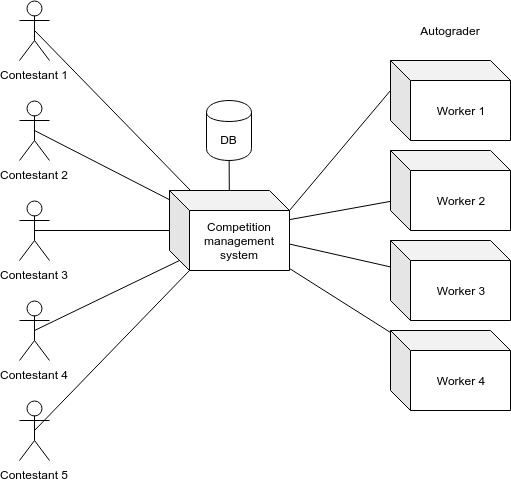
\includegraphics[width=0.45\textwidth]{images/paper-architecture-old.jpeg}}
\caption{Common Online Judge Architecture.}
\label{architecture-old}
\end{figure}

In order to grade contestants' submissions, online judge system has a subsystem called autograder. Contestants' submissions which are source code in a certain programming language will be graded by the autograding system by compiling the program and executes compiled program using test-cases that have been prepared by juries or problem setter. According to \cite{jordanioi}, this grading method is called black-box grading. By using the autograding system, the grading process can be done automatically and juries do not have to evaluate contestants' submissions manually. In order to increase the number of contestants' submissions in a certain amount of time, juries usually deploy autograder in many computers. Fig. \ref{architecture-old} depicts the architecture of common online judge system. In order to run autograder in many computers, the juries need to prepare many computers with the same specification to keep the fairness of the grading process.

Currently, almost every competitive programming competition uses online judge system to support the competition and use many computers to run autograder in order to improve grading performance, i.e., the number submissions graded in a certain amount of time. Every computer that runs autograder is called a worker. Even though autograder deployed in many computers, the grading performance often not enough to evaluate contestant solutions in real-time because the number of contestants is increasing. Furthermore, the number of computers to deploy autograder affect the procurement cost that need to be incurred by the juries. Therefore, a new grading system is needed to increase grading performance without increasing procurement cost that needs to be incurred.

When competing in a competitive programming competition, the contestants usually use their personal computer to write the solutions. Every contestants' computers usually have sufficient specification to compile and execute contestants' submissions. Therefore, contestants' computers have the ability to run the autograder program and evaluate contestants' submissions.

\section{Related Work}

There are some online judge systems that have been widely used to organize competitive programming competition. Some online judges offer other additional features like discussion forum, training gate, and rating system. Nowadays, most of the online judges are deployed as a web application and use a specific computer to grade contestants' submissions. There are many types of competitive programming competition rules. Most of the online judges only support a specific competition rule.

One of the most widely known competitive programming competition is ACM-ICPC (icpc.baylor.edu) competition where the competition uses ICPC rules. In ACM-ICPC competition, contestants compete in a group of three people. Every group has the same amount of problems to solve, and the score is determined by the number of solved problem and time penalty. There are many online judges that support this competitive programming rule. One of the online judges that support this type of competition is DOMJudge. DOMJudge is used in ACM-ICPC world final because it has many useful features, easy to use and open source.

Currently, most of the online judges use autograder to evaluate contestants' submissions. According to \cite{danutamalms}, autograder is a system that compiles, executes and evaluates source code. Evaluating source code manually takes three minutes while using autograder only need ten seconds. By using autograder, contestants can receive grading feedback faster and reduce the work that needs to be done by juries. Basically, the autograder evaluates the source code by compiling the source code and executing the compiled program using predefined test-cases. The output of contestant's solution program is compared to the predefined test-case and then graded. This evaluation method is called black-box grading \cite{jordanioi}.

The security aspect need to be considered when developing an autograding system. Competitive programming contestants might submit a source code that contains a dangerous code. According to \cite{wasikojsurvey}, there are several attacks that can be made by contestants, such as submitting compile bomb code, submitting code that destroys the autograder environment and submitting code that access forbidden computer's resource. In order to prevent such things, an autograding system must execute contestant's code in an isolated environment called sandbox.

There are several ways to create an isolated environment such as using virtual machine and containerization. By using a virtual machine, one can create an isolated operating system inside the host computer. The virtual machine uses a hypervisor to emulate computer hardware and run its own operating system. In Linux based operating system, there is a feature called KVM that makes it possible to create hypervisor as a process in Linux \cite{wfeltervmcontainer}. The virtual machine can be used to isolate the execution of contestant's code. However, by using the virtual machine, there is booting process that need to be done everytime contentant's submission is evaluated. This booting process takes so much computer's resource and reduces grading performance.

Another way to create an isolated environment is by using a container. A container is different from a virtual machine. A container gives isolation in software level without any hypervisor \cite{merkeldocker}. By using a container, the execution process can be done without booting a new operating system. The container works by using some Linux features such as chroot, namespace and cgroup. By using chroot, the filesystem of Linux process can be isolated \cite{lessardchroot}. The container uses a Linux feature called cgroup to limit process resources. By using cgroup, the memory usage, CPU usage, and disk IO usage of running process can be limited \cite{wfeltervmcontainer}. In order to hide other processes, user, and network from a running process, the container uses a Linux feature called namespace. By using a namespace, the Linux process can be isolated from from other processes, so the running process will not aware of the existence of other processes. Instead of a virtual machine, most of the autograding systems use container to isolate the grading process. This method was chosen because it is lighter and faster than the virtual machine. 

\section{Proposed Solution}

\subsection{Time and Memory Measurement}

In competitive programming competition, every problem has time and memory constraints. Contestants are asked to solve the problem by writing a program that satisfies the constraints. According to ICPC rules, when contestant's solution exceeds the problem constraints, the solution is rejected and the contestant gets a time penalty. Thus, the autograding system needs to tell whether contestant's solution exceeds the constraints or not. The problem is, every computer has a different performance when executing a program. The same program might run faster in one computer and slower in another computer. Currently, most of the online judge systems uses identical computers to evaluate contestants' submissions. By using identical computers, the same program is expected to run at the same duration and consume the same amount of memories.

Contestants' computers have different specification and performance. The juries cannot force the contestants to have an identical computer. Thus, a new time and memory measurement method is needed. The performance of a computer can be determined by its specifications such as CPU clock speed and operating system. However, besides CPU clock speed and operating system, there are so many other factors that affect computer performance such as temperature, cache size, the program itself, and many other factors. Thus, determining computer performance by its specification is very hard and not feasible to do.

\begin{equation}\label{tolerance-factor}
R_{contestant} < (1 + \gamma) \times R_{jury}
\end{equation}

In this work, the contestant's solution and jury's solution are compared. Contestant's solution is considered satisfying the problem constraints when the memory and CPU usage of contestant's solution is not exceeding jury's solution. Sometimes, contestant solution's memory or CPU exceeds the jury's solution a little bit because of the different implementation. The tolerance factor ($\gamma$) was added to tolerate this problem. Contestant's solution will be considered satisfying problem constraints when the Equation \ref{tolerance-factor} is fulfilled. When evaluating contestant's solution, the worker compils and executs contestant's solution and jury's solution. After executing the solutions, the worker compares the memory and CPU usage of the execution and determine whether the contestant's solution is satisfying problem constraints. 

\subsection{Load Balancing}

In order to increasing the grading performance, the grading jobs needs to be distributed evenly to the workers. There are several load balancing methods that can be used to distribute grading jobs evenly. The easiest way to distribute the jobs is by making each contestant to grade their own submissions. This method wasn't used in this work because this method creates security vulnerabilities.

The other way to distribute grading jobs is by using push-based load balancing method. In push-based load balancing, the online judge server chooses the worker to do the grading jobs. By using this method, every contestant does not know which submission they grade, thus can increase system security. To improve system security, every submission can be graded multiple times. In order to implement this method, the status of all workers are needed. This method is pretty hard to implement because the load balancer need to poll the worker status periodically and choose the best worker to evaluate the contestants' submissions.

\begin{figure}[htbp]
\centerline{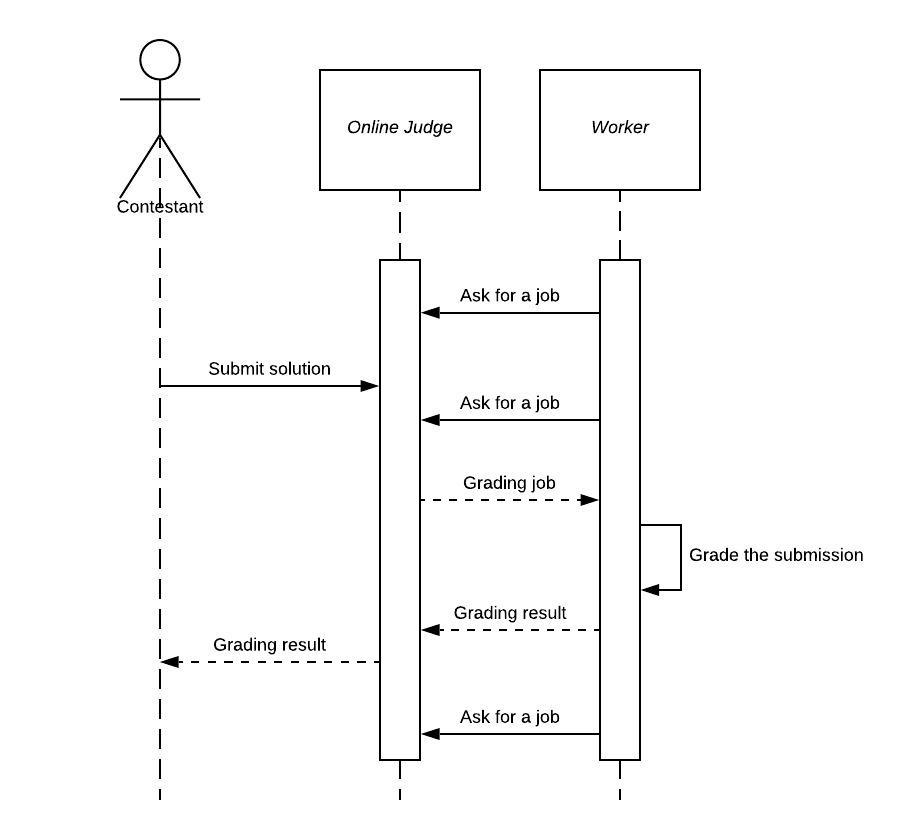
\includegraphics[width=0.5\textwidth]{images/paper-pull-based-load-balancing.jpeg}}
\caption{Pull-based Load Balancing.}
\label{pull-based-load-balancing}
\end{figure}

In this work, the pull-based load balancing method was chosen. By using this method, the worker status doesn't need to be polled periodically. The worker polls the jobs from the server periodically and evaluates them when there is a ready job that need to be evaluated. To improve system security, every submission is graded multiple times. A grading size of the system is defined as the number of second the autograder need to grades each submission. Fig. \ref{pull-based-load-balancing} depicts this method mechanism. This method is easier to be implemented than push-based load balancing method and has the same advantages.

\subsection{Evaluating Submission In Isolated Environment}

\begin{figure}[htbp]
\centerline{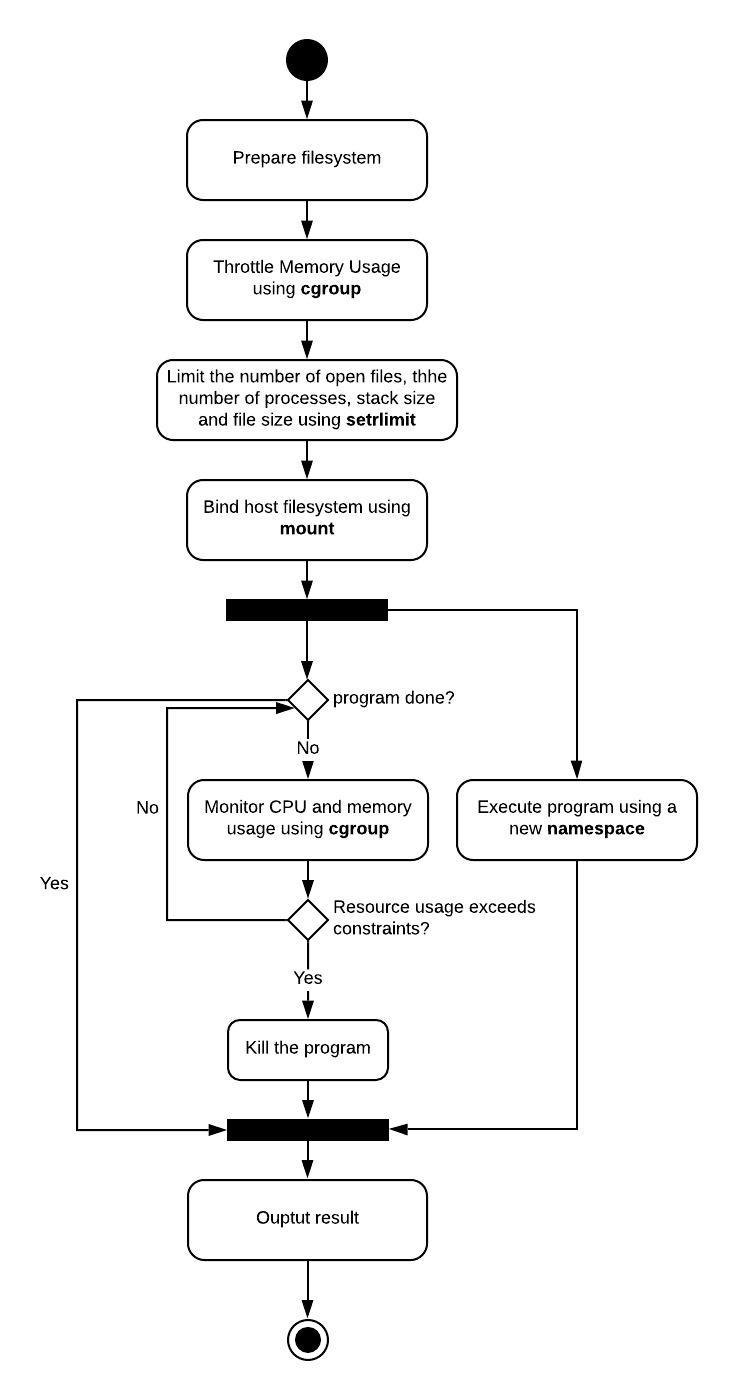
\includegraphics[width=0.5\textwidth]{images/paper-sandbox-activity.jpeg}}
\caption{Sandbox Activity Diagram.}
\label{paper-sandbox-activity}
\end{figure}

In order to isolate the evaluation process, a containerization method was chosen. The contestant's submission is compiled and executed inside a lightweight container. This container was created by using several Linux features and system calls such as cgroup, namespace, chroot and setrlimit. Cgroup is used to monitor and limit the CPU and memory consumption of the running process. The worker will kill the program when the CPU or memory usage is exceeding the limit. In order to isolate the host's user, process and network, a Linux feature called namespace is used. By using a namespace, the processes inside an isolated environment will not aware of any process, user or network in the outside of its own environment. In order to isolate the filesystem of a process, the chroot system call is used. Besides isolating the filesystem, some files from the host environment are also need to be brought into the isolated environment. Some of the host filesystems are brought into the isolated environment by using the mount system call. Some of processes resources are also limited by using the setrlimit system call. By using setrlimit system call, some process resources are limited such as the number of child processes, the stack size, the number of open files and the size of the created file of that process. Fig. \ref{paper-sandbox-activity} depicts how an isolated environment is created.

\subsection{Program Compilation}

In order to evaluated contestant's submissions, The submitted source code needs to be compiled and executed. A specific compiler is needed to compiles the source codes. Every worker should have the same version of the compiler. The same compiler with different version can produce different output. In order to keep the fairness of the grading process, the same version of the compiler needs to be distributed to all workers in the system. In this work, the compiler was installed in the autograder program and distributed to every worker. Every worker compiles the source code inside an isolated filesystem that has been installed with the same version of compilers.

\subsection{Obtaining Problem Test-cases}

Every worker needs test-cases to evaluate contestant solutions. A test-case is a pair of text files that contain input and output of the problem. Usually, the test-case files are generated by a test-case generator that has been created by the problem setters. The worker evaluates the contestant solution by executing the solution using the input test-case and compare the output with the output test-case. In order to evaluate the contestant solutions, the problem test-cases need to be brought into the worker. Bringing the test-cases into the worker is not easy because the test-case file can be a very large file and confidential.

In this work, the raw test-case is not transferred to all the workers. Transferring raw test-case files needs a huge bandwidth and can reduce grading performance. Instead of transferring raw test-case file, the test-case generator program is transferred to generate test-case files. The worker receives the test-case generator source code from the server and compiles it. The compiled test-case generator program then executed to generates input test-case. The worker uses the jury's solution to generates output test-case files. The worker also needs a checker program to compare contestant's output with jury's output. The checker program receives contestant's output and jury's output as its input and gives the verdict of the submission.

In order to hide the test-case information, the test-case generator program and the generated test-case files is encrypted. Even though the test-case is encrypted, the contestants might decrypt it if they know the encryption key. The contestant can attack the autograder program using reverse engineering technique to obtain the encryption key. In this work, this problem wasn't handled. Further research is needed to solve this problem.

\subsection{Handling Reverse Engineering Attacks}

Because the autograder programs are deployed in the contestants' computers, the contestants can do everything to the program. The contestant can attack the autograder program on their computer. There are many kinds of attacks that the contestant can do such as changing the compiler program, sending the false verdict to the server and refusing to grade other contestants' submissions. In this work, this kind of attacks weren't handled, but there is a way to handle this kind of attacks.

The autograder can prevent a contestant to refuse to do the grading process by monitoring the grading process. When it finds out that there is a worker that do not ask for a job for a long time or do not send the grading result for a long time, it can tells that there is a contestant that attacks the autograder program in their computer. Then, it can warns or disqualify the contestant for attacking the autograder program.

By grading every submission multiple times, a worker can be prevented from being attacked that cause it gives the wrong verdict after grading. When the autograder grades a submission multiple times and there is a contestant that attacks the autograder in their computer, it can tell by investigating the grading result. If the grading result of a worker is different from the rest of the workers, it can tell that the contestant is attacking the autograder program in that worker. Then, it can warn or disqualify that contestant for attacking the autograder program.

There are many more types of attacks that weren't handled in this work such as stealing jury's solution, other contestant's solution, and test-case generator. Even though that problems were not handle some type of attacks, this system can still work in several competitions such as ACM-ICPC. In ACM-ICPC, every team is given a computer by the juries to solve the problems. The juries can install the autograder program inside contestant's computer using the root user and not giving the root access to the contestant. By using this mechanism, the contestant cannot attack the autograder program inside their computer.

\section{Implementation}

\begin{figure}[htbp]
\centerline{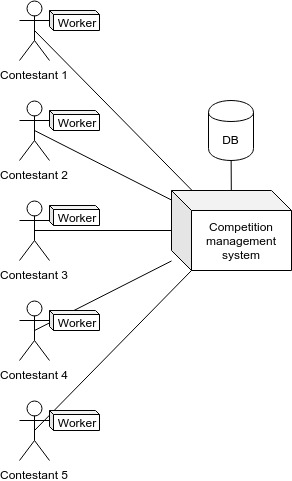
\includegraphics[width=0.4\textwidth]{images/paper-architecture-new.jpeg}}
\caption{Architecture of UGrade Online Judge.}
\label{architecture-new}
\end{figure}

Currently, most of online judge systems use separate computers to work as the worker of autograder. In order to improve the grading performance of the grading process, the contestant's computer is used as the worker of autograder. Fig. \ref{architecture-new} depicts the architecture of the system developed in this work. 

This system was named UGrade and implemented by developing five programs, i.e., UGServer, UGDesktop, UGCtl, UGJob, and UGSbox. UGServer handles everything related to competition such as authentication, contest creation, problem creation, etc. UGServer can be considered as a server of all the workers in the system. UGServer stores all the problems, submissions and the grading results. UGServer was developed using Python with Django and use GraphQL for the API. Django was used because of its ease of use.

To create an isolated environment, a sandbox utility program called UGSbox was created. By using UGSbox, one can execute a program inside an isolated environment and limit its resources. UGSbox was developed using Golang because of its ease of use. UGSbox is used by autograder program to compiles and executes the program for the grading process.

In this work, the autograder program was named UGJob. UGJob asks UGServer for a job and does the grading process. UGJob uses UGSbox to compiles and executes the source code it receives from UGServer. UGJob was developed using Golang because of its ease of use. The UGJob is deployed in every contestants' computers. Every installation of the UGJob is equipped with the same compiler to keep the fairness of the grading process.

\begin{figure}[htbp]
\centerline{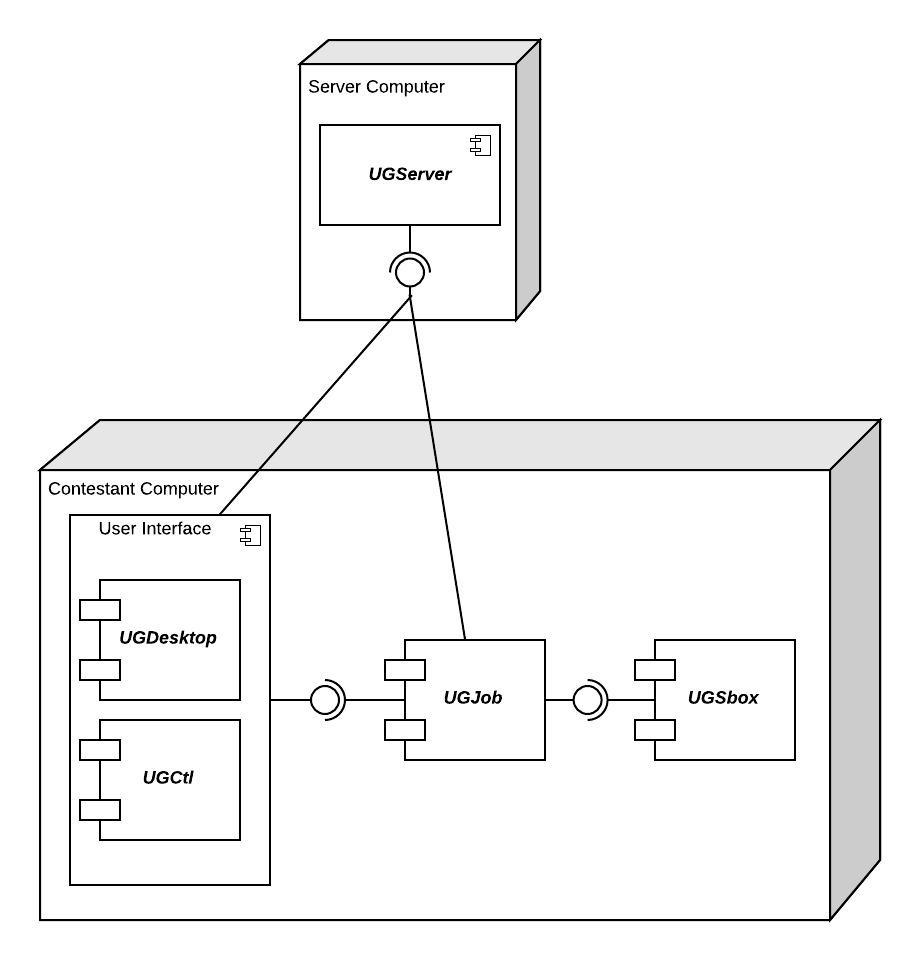
\includegraphics[width=0.4\textwidth]{images/paper-component.jpeg}}
\caption{Component Diagram of UGrade}
\label{component}
\end{figure}

The contestants can interact with the system using user interface programs, e.g., UGDesktop and UGCtl. UGDesktop is a graphical user interface program to interact with this system. Every contestant uses UGDesktop to read the problem and submit their solutions. UGDesktop executes UGJob periodically to grade the available job in the server. UGCtl is a text-based user interface program to interact with this system. Basically, UGDesktop and UGCtl have the same role in this system. UGCtl was developed just to automate the testing process. Fig. \ref{component} depicts the relationship of the components that developed in this work.

\section{Result and Analysis}

The grading performance between UGrade and DOMJudge was compared. DOMJudge was chosen as the comparison because it is open source and has been used in many competitive programming competitions. UGrade and DOMJudge were deployed on a computer with the same specification. Then fifteen computers were deployed to simulating the contestant actions. For DOMJudge, two more computers were deployed to work as the autograder worker. The number of two were chosen based on the Arkavidia competition where there were six workers for one hundred contestants, so approximately one worker is enough to handle fifteen contestants. For UGrade, the contestants act as a worker so there are fifteen computers worked as workers.

A dummy competition was created with a single problem, e.g., polynomial multiplication. This problem was expected to be solved using $O(N log N)$ solution, but there are many other solutions with different complexity. Four types of solution were used to simulating contestant submission. The first and second type of solution have $O(N^2)$ complexity but have a different implementation. The third solution has $O(N^{log_2{3}})$ complexity. The fourth solution has $O(N log N)$ complexity and considered as the correct solution.

\begin{table}[ht!]
    \label{grading-time}
    \caption{Average Time to Grade A Single Submission.}
    \begin{center}
        \begin{tabular}{| c | c |}
    \hline
    System & Time (seconds) \\
    \hline
    \hline
    DOMJudge & 198.0845733 \\
    \hline
    UGrade with one as grading size & 12.3706562 \\
    \hline
    UGrade with two as grading size & 11.42285704 \\
    \hline
    UGrade with five as grading size & 14.21330876 \\
    \hline
\end{tabular}
    \end{center}
\end{table}

The fifteen computers were submitting each type of solution one by one two times. Every event that happens on the system was logged and the result was analyzed. In this work, every submission was graded multiple times for UGrade system. UGrade was tested nine times using three different grading size, e.g., one, two and five. The average time to grade a single submission in DOMJudge and UGrade was calculated. Table \ref{grading-time} shows the comparison between the average time to grade a single submission in each test. Based on Table \ref{grading-time}, it can be known that the UGrade grades the submission faster than DOMJudge. It can also be known that the grading size of UGrade affects the grading performance a little bit. By increasing the grading size of UGrade, each submission would be graded slower because each submission needs to be graded many times when the grading size is high. In the other hand, increasing the grading size will increase the system security because the submission graded in many workers. The juries need to adjust the grading size so it is fast enough to grade a single submission and secure enough to prevent any attacks from contestants.

\section{Conclusion}

Based on the development and testing that have been done, there are some lessons that can be learned.
\begin{enumerate}
    \item There is a high grading performance improvement in UGrade compared to many online judges that  currently exists. This performance improvement is caused by the number of the worker in the UGrade which follows the number of contestants in the competition.
    \item The grading performance of UGrade is not affected by the number of contestants but affected by the grading size number of UGrade. The high number of contestant causes a high number of worker too, so that does not affect the grading performance. However, the grading size number causes the number of submission doubles, thus affects the grading performance.
    \item The high number of grading size reduces grading performance but increases system security. The low number of grading size increases grading performance but reduces system security. The juries need to adjust the grading size to achieve the best result.
    \item UGrade can keep the fairness of grading process even if the worker computers have different specification and performance. UGrade achieves this by comparing the jury's solution and contestant's solution in the same computer.
\end{enumerate}

\section{Further Work}

The UGrade online judge system still cannot handle some type of attacks such as test-case stealing, solution stealing and reverse engineering attacks. Some of the reverse engineering attacks can be handled by monitoring the grading process of the system. In order to handle test-case stealing, solution stealing and some other type of attacks, further research is needed to improve the security aspect of this system. 

In this work, a pull-based load balancing technique was used to distribute the grading work to all of the workers. This technique has caused UGServer load to become very huge and decrease grading performance. In order to increase the grading performance and reduce the load of UGServer, further research is needed to find another way to do the load balancing process.

\begin{thebibliography}{00}

\bibitem{uriojpaper} J. L. Bez, N. A. Tonin, and P. R. Rodegheri, ``URI Online Judge Academic: A tool for algorithms and programming classes,'' \textit{2014 9th International Conference on Computer Science \& Education}, 2014.
\bibitem{wasikojsurvey} S. Wasik, M. Antczak, J. Badura, A. Laskowski, and T. Sternal, ``A Survey on Online Judge Systems and Their Applications,'' \textit{ACM Computing Surveys}, vol. 51, no. 1, pp. 1–34, 2018.
\bibitem{wfeltervmcontainer} W. Felter, A. Ferreira, R. Rajamony, and J. Rubio, ``An updated performance comparison of virtual machines and Linux containers,'' \textit{2015 IEEE International Symposium on Performance Analysis of Systems and Software (ISPASS)}, 2015.
\bibitem{danutamalms} K. Danutama and I. Liem, ``Scalable Autograder and LMS Integration,'' \textit{Procedia Technology}, vol. 11, pp. 388–395, 2013.
\bibitem{merkeldocker} D. Merkel, ``Docker: Lightweight Linux Containers for Consistent Development and Deployment,'' \textit{Linux J.}, vol. 2014, no. 239, Mar. 2014.
\bibitem{lessardchroot} P. Lessard, ``InfoSec reading room report: Linux process containment - a practical Look at chroot and user mode Linux,'' \textit{SANS Institute}, 2003.
\bibitem{jordanioi} J. Fernando and I. Liem, ``Components and Architectural Design of an Autograder System Family,'' \textit{Olympiads in Informatics}, vol. 8, pp. 69–79, Jan. 2014.

\end{thebibliography}

\end{document}
